\documentclass{article}
\usepackage[tc]{titlepic}
\usepackage{xcolor}
\usepackage{graphicx}
\usepackage{tipa}
\usepackage{pagecolor,lipsum}
\usepackage{amsmath}
\usepackage{amsfonts}

\usepackage{amssymb}
\usepackage{amsthm}
\usepackage{centernot}
\usepackage{xcolor}
\usepackage{listings}
\usepackage{tikz}
\usetikzlibrary{calc}

\newtheorem{theorem}{Theorem}
\newtheorem{defintion}{Definition}
\newtheorem{collorary}{Collorary}
\newtheorem{example}{Example}
\newtheorem{remark}{Remark}
\newtheorem{note}{Note} 

\begin{document}
\section{Algorithms are important for interview}
\begin{enumerate}
\item Quick Sort 
    \begin{itemize}
    \item The average runtime is $\mathcal{O}(n\log{}n)$
    \item The worst case is $\mathcal{O}(n^2)$
        \begin{itemize}
        \item Given an array $[1, 2, 3, 4]$, choose the right most element as \\ 
              pivot which is [4] $=>$ [1, 2, 3][4] $=>$ [1, 2][3] $=>$ [1][2]
        \item How to choose the pivot is critical.
        \end{itemize} 
    \item Memory space is $\mathcal{O}(1)$ 
    \item Untable sort and Stable sort
        \begin{itemize}
        \item If the keys keep the same relative orders after keys are sorted \\ 
              then the sort algorithm is stable. Otherwise it is unstable. \\\\
              Sort the second coordinates \\ 
               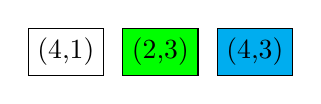
\begin{tikzpicture}
                \coordinate (s) at (0,0);
                  \node[minimum size=6mm, draw, rectangle] at (s) {(4,1)};
                \coordinate (s) at (1.2,0);
                  \node[minimum size=6mm, fill=green, draw, rectangle] at (s) {(2,3)};
                \coordinate (s) at (2.4,0);
                  \node[minimum size=6mm, fill=cyan, draw, rectangle] at (s) {(4,3)};
              \end{tikzpicture} \\

              Sort the first coordinates [stable sort]\\
               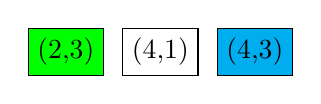
\begin{tikzpicture}
                \coordinate (s) at (0,0);
                  \node[minimum size=6mm, fill=green, draw, rectangle] at (s) {(2,3)};
                \coordinate (s) at (1.2,0);
                  \node[minimum size=6mm, draw, rectangle] at (s) {(4,1)};
                \coordinate (s) at (2.4,0);
                  \node[minimum size=6mm, fill=cyan, draw, rectangle] at (s) {(4,3)};
              \end{tikzpicture} \\

              Sort the first coordinates [unstable sort]\\
               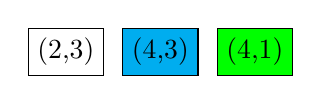
\begin{tikzpicture}
                \coordinate (s) at (0,0);
                  \node[minimum size=6mm, draw, rectangle] at (s) {(2,3)};
                \coordinate (s) at (1.2,0);
                  \node[minimum size=6mm, fill=cyan, draw, rectangle] at (s) {(4,3)};
                \coordinate (s) at (2.4,0);
                  \node[minimum size=6mm, fill=green, draw, rectangle] at (s) {(4,1)};
              \end{tikzpicture} \\
        \end{itemize} 
        \item Unstable Sort 
            \begin{itemize}
            \item Quick Sort 
            \item Heap Sort
            \end{itemize} 
        \item Stable Sort 
            \begin{itemize}
            \item Merge Sort 
            \item Selection Sort 
            \end{itemize} 
    \end{itemize} 
\item Find the Kth smaller element in a given array in $\mathcal{O}(n)$
\item Merge Sort, 
    \begin{itemize}
    \item The average and worst runtime is $\mathcal{O}(n\log{}n)$ 
    \item Stable sort
    \end{itemize} 
\item Max distance for $j - i$ given $arr[j] > arr[i$] 
\item Single linked list
    \begin{itemize}
        \item reverse, iteration, recursion
        \item remove, 
        \item insert to sorted list 
        \item clone list
        \item check circular linkedlist 
    \end{itemize} 
\item Double linkedlist
    \begin{itemize}
        \item remove node
        \item insert node
        \item append node
    \end{itemize} 
\item Eight queen problem
\item Sudoku Solver problem
\item Connected island 
\item Serialize Binary Tree 
    \begin{itemize}
    \item Use technic similar to implementations of heap with array  
    \end{itemize} 
\item Serialize general tree 
\item Tree Traveral
    \begin{itemize}
    \item preorder  
        \begin{itemize}
        \item use it to serialize Binary Tree, postorder can be deserialized BT.
        \end{itemize} 
    \item inorder 
    \begin{itemize}
    \item Check if a Binary Tree is Binary Search Tree   
    \end{itemize} 
    \item postorder
    \item levelorder 
\end{itemize} 

\item Rotate square array
\item Print rectangle array in spiral shape.
\item Multiply long integers using array 
\item Find the maximum elements from sorted array are shifted
\item Find the minimum elements from sorted array are shifted
\item Dynamic Programming
    \begin{itemize}
     \item maximum continuous sum in $\mathcal{O}(n)$ 
     \begin{itemize}
     \item how to support negative number
     \item print the indexes out 
     \end{itemize}
     \item maximum non-continuous sum $\mathcal{O}(n)$ 
     \item multiply all the elements in an array except current element $\mathcal{O}(n)$ 

    \end{itemize}

\item Graphic Problem
\begin{itemize}
 \item find a path from two nodes 
 \item find the shortest path from two nodes
 \item find the minimum weight path from two nodes
 \item how to find the loop in a graph
 \item find all the neighbours which are kth distance from a given node
\end{itemize}

\item How to represent a Graph
\begin{itemize}
 \item adjecent matrix 
 \item adjecent list
 \item What is the different between the two data structures
\end{itemize}

\item BackTracking
    \begin{itemize}
     \item Coin Change problem.
     \begin{itemize}
      \item find the minimum number of coins [shortest path from the root]
      \item find the maximum number of coins [longest path from the root]
      \item dynamic programming with HashMap 
     \end{itemize}
     \item Eight Queen Problem
     \item Sudoku Solver
     \item Find the maximum number of connected dots in an 2d array 
     \item Find the path from one word to other word which only one letter can be changed to a valid dictionary word every step.(Facebook question) 
    
    \end{itemize}

\item Binary Tree
    \begin{itemize}
    \item Check a Binary Tree is Binary Search Tree 
    \begin{itemize}
     \item recursion technic
     \item defintion technic 
    \end{itemize}

    \item Check whether two Binary Tree are isomorphic
    \item Find the mirror of a Binary Tree
    \item Find the longest path in a Binary Tree
    \item Print all the paths in a Binary Tree
    \item Find the maximum sum of path in a Binary Tree
    \item Invert a Binary Tree
    \item Binary Tree to linkedlist
        \begin{itemize}
        \item Binary Tree to circular double linked list [hard]
        \item Binary Tree to single linked list with one queue
        \item Delete whole tree
        \begin{itemize}
        \item Use two queues 
        \item Post order traveral
        \item Use memory space $\mathcal{O}(1)$
        \begin{itemize}
        \item Move one branch to branch 
        \end{itemize} 
        \end{itemize} 
        \end{itemize} 
    \end{itemize} 
\end{enumerate} 

\end{document}
